\chapter{Transmisión de datos}

\section{Sistema de Empaquetado RTP}

RTP es la abreviación de \textit{Real-Time Transport Protocol}, por su denominación en inglés. Es un protocolo de nivel de sesión utilizado para la transmisión de información en timpo real, como por ejemplo, audio y video en una video conferencia.  En aplicaciones de \textbf{Voz sobre IP}, \textbf{RTP} es el protocolo responsable de la transmisión de los datos. Está desarrollado por el grupo de trabajo de transporte de audio y video del \textbf{IETF}.


\subsection{Características generales y estructura}
Aunque RTP tiene algunas características de protocolo de nivel de transporte (Según el modelo OSI), es transportado usando UDP, UDP no maneja sesiones ni mecanismos que garanticen la recepción de los paquentes, pero es usado por RTP en lugar de TCP debido a que reduce el tiempo de envío de los paquetes a través de la red. En aplicaciones de voz y video es más importante una transmisión rápida que la pérdida de algunos paquetes durante el recorrido.

La figura ~\ref{rtp} muestra la estructura del encabezado de un paquete de tipo RTP.

\begin{figure}[H]
\centering
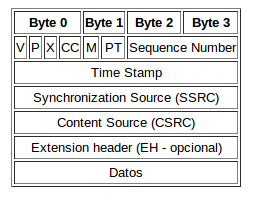
\includegraphics[width=7cm]{logos/rtp.png}
\caption{Encabezado de paquete RTP.}
\label{rtp}
\end{figure}


\begin{itemize}
\item Número de versión de RTP (V - versión number): 2 bits. La versión definida por la especificación actual es 2.

\item Relleno (P - Padding): 1 bit. Si el bit del relleno está activado, hay uno o más bytes al final del paquete que no es parte de la carga útil. El último byte del paquete indica el número de bytes de relleno. El relleno es usado por algunos algoritmos de cifrado.

\item La extensión (X - Extensión): 1 bit. Si el bit de extensión está activado, entonces el encabezado fijo es seguido por una extensión del encabezado. Este mecanismo de la extensión posibilita implementaciones para añadir información al encabezado RTP.

\item Conteo CSRC (CC): 4 bits. El número de identificadores CSRC que sigue el encabezado fijo. Si la cuenta CSRC es cero, entonces la fuente de sincronización es la fuente de la carga útil.

\item El marcador (M - Marker): 1 bit. Un bit de marcador definido por el perfil particular de media.

\item Tipo de Carga útil (PT - Payload Type): 7 bits. Un índice en una tabla del perfiles de media que describe el formato de carga útil. Los mapeos de carga útil para audio y vídeo están especificados en el RFC 1890.


\item El número de Secuencia: 16 bits. Un único número de paquete que identifica la posición de este en la secuencia de paquetes. El número del paquete es incrementado en uno para cada paquete enviado.

\item 
Sellado de tiempo: 32 bits. Refleja el instante de muestreo del primer byte en la carga útil. Varios paquetes consecutivos pueden tener el mismo sellado si son lógicamente generados en el mismo tiempo - por ejemplo, si son todo parte del mismo frame de vídeo.
\item 
SSRC: 32 bits. Identifica la fuente de sincronización. Si la cuenta CSRC es cero, entonces la fuente de carga útil es la fuente de sincronización. Si la cuenta CSRC es distinta a cero, entonces el SSRC identifica el mixer(mezclador).

\item  CSRC: 32 bits cada uno. Identifica las fuentes contribuyentes para la carga útil. El número de fuentes contribuyentes está indicado por el campo de la cuenta CSRC; Allí puede haber más de 16 fuentes contribuyentes. Si hay fuentes contribuyentes múltiples, entonces la carga útil son los datos mezclados de esas fuentes.


\item EH: El tamaño de este dato debe ser CC*32 en bits.

\item Datos: El tamaño de los datos debe ser de X *((EHL+1)*32) donde EHL es la longitud de la extensión del la cabecera en unidades de 32 bits.

\end{itemize}

\begin{verbatim}
http://en.wikipedia.org/wiki/Real-time_Transport_Protocol

http://es.wikipedia.org/wiki/User_Datagram_Protocol

\end{verbatim}



\section{Códigos de longitud variable}

